% ch01-ml.tex -- Chapter 1: Data as matrices
\chapter{Data as matrices: NumPy and the dataset}\label{ch:data}

Every model in this book begins the same way: a table of numbers. Rows are
things that happened --- a penguin measured, a transaction approved, a pixel
grid flattened --- and columns are the measurements we chose to record. Before
we can fit anything, we have to get that table out of a file, into memory, and
into a shape a computer can multiply. That is the whole job of this chapter.
You will learn to see a dataset as one matrix $X\in\mathbb R^{n\times d}$, to
load it from a CSV with nothing but the standard library and NumPy, to encode
categories as columns, to shuffle and slice it into training pieces, and to do
all of that fast enough that you never think about it again. More importantly,
you will learn where it goes wrong: the missing cells, the impossible values,
and the duplicated rows that quietly inflate your results. Nothing here is
glamorous. All of it is load-bearing.

% from-zero:why:begin
\paragraph{Why this exists.} Some rules are impossible to write down by hand: what
makes an email spam, or a photo a cat. Machine learning replaces the hand-written rule with examples and a method
that finds the rule for you. Every such method needs the examples in the same form, a table of numbers, and
the first job of a practitioner is getting data into that form and checking that it is sound. A model built
on a badly loaded table is wrong in ways no later technique can repair.
% from-zero:why:end

% from-zero:begin
\begin{rulebox}[Before you start]
Basic Python: variables, lists, loops and functions. The \emph{Start here} chapter has a short Python primer, plus a one-page recap of the vectors and matrices this book calls on (from \textbf{Book~3, Chapter~2}). You do not need to have read Book~3 first.
\end{rulebox}
\begin{wins}[After this chapter you can]
\begin{itemize}
\item load a CSV file into memory and describe it as a matrix of samples by features;
\item use NumPy to compute with whole arrays at once, and explain broadcasting;
\item encode categories as numbers without inventing a fake order;
\item find duplicated, missing and impossible values before they quietly ruin a result.
\end{itemize}
\end{wins}
\begin{principle}[How to think about this]
Before any clever model, remember that a computer sees only numbers, so your first task is translation: rows are things, columns are measurements. Time spent checking the table (missing values, odd units, duplicates) is the best investment in machine learning, because a model will happily learn from mistakes.
\end{principle}
% from-zero:end

\section{Why datasets are matrices (and when they are not)}\label{sec:matrices}

A \emph{dataset}\index{dataset} is a collection of $n$ samples, each described
by the same $d$ measurements. Stacked into a table, the samples form the
\emph{design matrix}\index{design matrix} $X\in\mathbb R^{n\times d}$, one row
per sample: row $i$ is the transposed vector $\mathbf x_i^T$, and column $j$ is
\emph{feature}\index{feature} $j$ --- one number measured for every sample.
When the sample also carries an answer we want to predict, it lives in a
separate vector $\mathbf y$ of \emph{targets}\index{target}, aligned row-by-row
with $X$. Together $\mathcal D=\{(\mathbf x_i,y_i)\}_{i=1}^{n}$.

\begin{figure}[ht]\centering
\begin{tikzpicture}[scale=0.62]
  % design-matrix block diagram
  \draw[fill=amberbg] (4,0) rectangle (5,5);
  \draw[fill=accentsoft] (0,3) rectangle (6,4);
  \draw[step=1,black!35,very thin] (0,0) grid (6,5);
  \draw[thick] (0,0) rectangle (6,5);
  \node at (4.5,2.4) {\small};
  \node[font=\footnotesize] at (0.5,3.5) {$x_{i1}$};
  \node[font=\footnotesize] at (4.5,3.5) {$x_{ij}$};
  \node[font=\footnotesize] at (5.5,3.5) {$x_{id}$};
  \node[font=\footnotesize,anchor=east] at (-0.15,3.5) {row $i$: sample $\mathbf x_i^T$};
  \node[font=\footnotesize,anchor=south,rotate=90] at (4.5,5.25) {\,feature $j$};
  \draw[decorate,decoration={brace,amplitude=4pt,mirror}] (-0.3,0) -- (-0.3,5)
    node[midway,left=6pt] {$n$ samples};
  \draw[decorate,decoration={brace,amplitude=4pt}] (-0.3,5.35) -- (6.3,5.35)
    node[midway,above=6pt] {$d$ features};
  \node[font=\small] at (3,-0.9) {$X\in\mathbb R^{n\times d}$};
  % targets column
  \draw[fill=goodbg] (7.3,0) rectangle (8.1,5);
  \draw[step=1,black!35,very thin] (7.3,0) grid (8.1,5);
  \draw[thick] (7.3,0) rectangle (8.1,5);
  \node[font=\footnotesize] at (7.7,3.5) {$y_i$};
  \node[font=\small] at (7.7,-0.9) {$\mathbf y$};
  \draw[<->,dashed,slate] (6.15,3.5) -- (7.25,3.5);
\end{tikzpicture}
\caption{A dataset is a matrix. Row $i$ of the design matrix $X$ is one sample
$\mathbf x_i^T$; column $j$ is one feature measured for every sample. The
target vector $\mathbf y$ is aligned row-by-row: $y_i$ belongs to $\mathbf
x_i$.}\label{fig:design-matrix}
\end{figure}

This is a convention, not a law of nature, and it is a productive one. Once a
dataset is a matrix, \emph{scoring the whole dataset} is one matrix product
$X\mathbf w$; \emph{centring every column} is one subtraction; \emph{finding
the nearest class mean} is a broadcast and an $\arg\min$. The linear algebra
you built in Book 3 stops being notation and becomes executable.

When the convention breaks, it breaks for a reason. Text arrives as
variable-length sequences, not rows of equal width --- the sequence models of
chapter~10 inherit that problem. Images are grids, so a picture
becomes a $(C,H,W)$ tensor and flattening it into a row throws away the spatial
structure a convolution needs. Networks of interacting items (users,
molecules, flights) are graphs, not tables. None of that fits this chapter ---
and none of it is needed yet. Tabular data is the workhorse: surveys, sensor
logs, prices, medical measurements. Learn the matrix first.

\begin{principle}[The matrix is the contract]
\index{design matrix!as contract}
Every algorithm in this book expects the same deal: a 2-D \texttt{ndarray} of
shape $(n,d)$ whose rows are samples and columns are features, plus a 1-D
target vector of shape $(n,)$ when the task is supervised. When a method
misbehaves, check the contract first --- wrong shapes cause more bugs than
wrong maths.
\end{principle}

\section{NumPy arrays: shape, dtype, broadcasting}\label{sec:numpy}

NumPy's \texttt{ndarray}\index{ndarray} is a typed, rectangular block of
memory. Three attributes describe any array: \texttt{shape} (a tuple of axis
lengths, e.g.\ \texttt{(150, 4)}), \texttt{dtype} (the element type, e.g.\
\texttt{float64}), and \texttt{ndim} (how many axes). Two habits pay off
immediately:

\begin{itemize}
\item \textbf{Say the shape aloud.} \texttt{X.shape == (150, 4)} means 150
  samples, 4 features. The vast majority of array bugs are shape confusions,
  and they are loud if you listen.
\item \textbf{Watch the dtype.}\index{dtype} An \texttt{ndarray} is
  homogeneous: every element has the same type. Reading mixed text columns
  through \texttt{np.array} without care gives you \texttt{<U32} strings;
  writing a float into an \texttt{int} array silently truncates it
  (\S\ref{sec:mistakes}).
\end{itemize}

The feature that carries the whole book is
\emph{broadcasting}\index{broadcasting}: NumPy's rules for applying a binary
operation ($+$, $-$, $*$, $/$, comparisons) to arrays of different shapes.
Three rules, applied axis-by-axis from the right~\cite{npbroadcast}:

\begin{rulebox}[Broadcasting, three rules]
\begin{enumerate}
\item Align the two shapes on their \emph{trailing} (rightmost) axes; missing
  axes are treated as size 1.
\item Two dimensions are compatible if they are equal, or if one of them is 1.
\item A dimension of size 1 is \emph{stretched} (conceptually copied) along
  that axis. If any pair of aligned dimensions fails rule 2, NumPy raises
  \texttt{ValueError: operands could not be broadcast together}.
\end{enumerate}
\end{rulebox}

\begin{figure}[ht]\centering
\begin{tikzpicture}[scale=0.5]
  % (4,1) column vector
  \draw[step=1,black!35,very thin] (0,0) grid (1,4); \draw[thick] (0,0) rectangle (1,4);
  \node[font=\footnotesize] at (0.5,3.5) {2}; \node[font=\footnotesize] at (0.5,2.5) {0};
  \node[font=\footnotesize] at (0.5,1.5) {4}; \node[font=\footnotesize] at (0.5,0.5) {1};
  \node[font=\footnotesize] at (0.5,-0.7) {$(4{,}1)$};
  \node[font=\large] at (1.7,2) {$+$};
  % (1,3) row vector
  \draw[step=1,black!35,very thin] (2.4,3) grid (5.4,4); \draw[thick] (2.4,3) rectangle (5.4,4);
  \node[font=\footnotesize] at (2.9,3.5) {10}; \node[font=\footnotesize] at (3.9,3.5) {20};
  \node[font=\footnotesize] at (4.9,3.5) {30};
  \node[font=\footnotesize] at (3.9,2.3) {$(1{,}3)$};
  % stretch ghosts
  \draw[->,accent,thick] (3.9,4.3) -- (3.9,4.9);
  \draw[->,accent,thick] (0.5,4.3) -- (0.5,4.9);
  \node[font=\footnotesize,slate] at (3.4,5.3) {each size-1 axis stretches};
  \draw[->,thick] (6.0,2) -- (7.0,2);
  % (4,3) result
  \draw[step=1,black!35,very thin] (7.3,0) grid (10.3,4); \draw[thick] (7.3,0) rectangle (10.3,4);
  \node[font=\footnotesize] at (7.8,3.5) {12}; \node[font=\footnotesize] at (8.8,3.5) {22}; \node[font=\footnotesize] at (9.8,3.5) {32};
  \node[font=\footnotesize] at (7.8,2.5) {10}; \node[font=\footnotesize] at (8.8,2.5) {20}; \node[font=\footnotesize] at (9.8,2.5) {30};
  \node[font=\footnotesize] at (7.8,1.5) {14}; \node[font=\footnotesize] at (8.8,1.5) {24}; \node[font=\footnotesize] at (9.8,1.5) {34};
  \node[font=\footnotesize] at (7.8,0.5) {11}; \node[font=\footnotesize] at (8.8,0.5) {21}; \node[font=\footnotesize] at (9.8,0.5) {31};
  \node[font=\footnotesize] at (8.8,-0.7) {$(4{,}3)$};
\end{tikzpicture}
\caption{Broadcasting a $(4,1)$ column and a $(1,3)$ row: both size-1
dimensions stretch until the shapes agree, and the sum is $(4,3)$ --- an
\emph{outer} operation built from two inner-shaped pieces. The same mechanism
centres columns (\texttt{X - mu}), scales them (\texttt{(X - mu) / sd}), and
builds pairwise distance tables (\texttt{A[:, None, :] - B[None, :, :]}).
}\label{fig:broadcast}
\end{figure}

Read rule 3 as ``stretch, don't copy'': no data is duplicated in memory, which
is why broadcasting is both fast and memory-cheap --- and also why a mistaken
stretch is silent. The two traps that matter most in this book:

\begin{itemize}
\item $(n,1)+(1,d)\to(n,d)$ is \emph{intended} outer behaviour (Figure
  \ref{fig:broadcast}); $(n,1)+(n,)\to(n,n)$ is usually an accident --- a
  length-$n$ row and a length-$n$ column silently combine into a full $n\times
  n$ table. Fix by making the intended axis explicit: \texttt{b[:, None]}.
\item \texttt{X[:, None, :] - B[None, :, :]} inserts axes to build an
  $(n,m,d)$ intermediate --- correct, but memory-hungry for large $n\cdot m$
  (\S\ref{sec:vectorise}).
\end{itemize}

\begin{checkpoint}[Shapes by rules]
Apply the three rules on paper before running anything. What is
\texttt{np.ones((3,4))} \texttt{+} \texttt{np.arange(4)}? And
\texttt{np.ones((3,4))} \texttt{+} \texttt{np.arange(3)}? Which one fails
and why?
\end{checkpoint}

\section{Loading data: CSV \texorpdfstring{$\to$}{->} ndarray}\label{sec:loading}

A CSV is text: one row per line, fields separated by commas --- when you are
lucky. The standard library's \texttt{csv} module handles the unlucky cases
(quoted commas, blank cells); NumPy handles the rest. The pattern we will use
all book is \emph{parse to strings first, convert columns second}:
\texttt{csv.reader} gives a list of string rows; the feature columns become a
float \texttt{ndarray}; the label column stays strings.

\lstinputlisting[language=Python,caption={\texttt{code/ch01/load\_iris\_scratch.py}: CSV to $(X,\mathbf y)$ with the standard library --- no pandas --- followed by a seeded 80/20 split and a distance-to-mean classifier whose core is exactly eight lines.},label={lst:load-iris}]{code/ch01/load_iris_scratch.py}

Run from the repository root, it prints:

\lstinputlisting[numbers=none]{code/ch01/load_iris_scratch.out.txt}

\begin{example}[A classifier in eight lines]\label{ex:eight-lines}
Strategy: \emph{nearest class mean}. Compute each class's centroid on the
training rows, then assign each test row to its closest centroid.\par
\begin{solution}
Lines 24--31 of Listing~\ref{lst:load-iris} do exactly that. The only
mathematics is a mean and a distance; everything else is indexing. On the
seeded split it reaches $0.967$ test accuracy ($29/30$) --- a real number from
a real run, on Ronald Fisher's 1936 iris measurements~\cite{fisher1936}. The
point is not the accuracy; it is that ``a model'' is just shapes: $X$
$(150,4)$, centroids $(3,4)$, predictions $(30,)$.
\end{solution}
\end{example}

\subsection{Missing values and friends}\label{sec:missing}

Real files lie by omission. The \texttt{penguins} dataset --- 344 Antarctic
penguins measured at Palmer Station~\cite{gorman2014,seaborn-data} --- ships
with 19 empty cells: two penguins lack all four bill/flipper/mass
measurements, and nine more lack a recorded \texttt{sex}. Loading through
\texttt{float(...)} or \texttt{np.loadtxt} turns an empty field into an error
or a silent \texttt{nan}; either way, \textbf{your first act after loading is
counting what is missing}.

\lstinputlisting[language=Python,caption={\texttt{code/ch01/missing\_values.py}: count NaNs per column, then measure what each repair costs.},label={lst:missing}]{code/ch01/missing_values.py}

\lstinputlisting[numbers=none]{code/ch01/missing_values.out.txt}

\begin{example}[Drop, fill, or flag]\label{ex:missing}
Strategy: missingness is data too. For each column ask \emph{why} the cell is
empty before deciding what to do with it.\par
\begin{solution}
Listing~\ref{lst:missing} compares the two standard repairs on the four
numeric penguin columns. Dropping the two incomplete rows and filling them
with the column median barely move the column means (largest shift: body mass,
$4201.75\to 4200.87$) --- either is defensible \emph{here} because the holes
are tiny. The \texttt{sex} column is different: its 11 holes are 3\% of the
data and categorical, so there is no median to fill. We make \emph{missing}
its own category in \S\ref{sec:onehot} and let the model learn what it means.
The rule that survives: \textbf{choose the repair that loses the least
information}, and record whichever you chose --- a reviewer will ask.
\end{solution}
\end{example}

\begin{figure}[ht]\centering
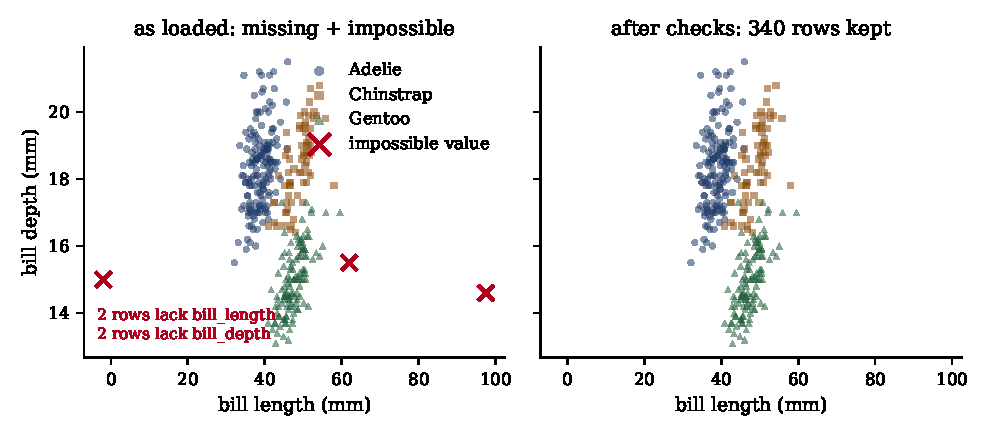
\includegraphics[width=\linewidth]{figures/ch01/missing_scatter.pdf}
\caption{Bill length vs bill depth for the \texttt{penguins} dataset
(\texttt{figures/fig\_ch01\_missing\_scatter.py}). Left: as loaded --- three
impossible bill lengths injected for the hygiene demo plot as red crosses (one
stretches the axis so far the real data compresses), and two rows that lack
\emph{both} coordinates cannot be drawn at all. Right: the same data after the
checks of \S\ref{sec:hygiene}.}\label{fig:missing-scatter}
\end{figure}

\subsection{Encodings, and leakage at the loading step}\label{sec:loadleak}

Two more things a raw column can hide. \emph{Encoding drift}: the same fact
spelled \texttt{MALE}, \texttt{Male}, \texttt{m}, and \texttt{male} lands as
four categories --- normalise case and whitespace \emph{before} building any
codebook. And the sneakiest failure of all:
\emph{leakage}\index{leakage} --- information from the future (the test rows)
flowing into the decisions you make on the past (the training rows). At the
loading step three leaks recur:

\begin{enumerate}
\item \textbf{Normalize-then-split}: computing column means/standard
  deviations on the full file, then splitting. The test rows contributed to
  the scaling --- a small but real leak. Fit statistics on the training rows
  only~\cite{sklearnpitfalls}.
\item \textbf{Split-then-dedup}: removing duplicates \emph{after} the split,
  so a row and its twin can land on opposite sides and give the model a free
  answer. \S\ref{sec:hygiene} measures what this costs.
\item \textbf{Codebook-from-everything}: building the one-hot level list (or a
  vocabulary) from all rows including held-out ones. Usually a small leak;
  occasionally the held-out level simply does not exist in training and the
  bug hides until deployment.
\end{enumerate}

The test set must look like the future. Anything your pipeline learns ---
means, medians, category lists, the decision to drop a column --- it must
learn from training rows alone.

\section{Features and targets; one-hot encoding}\label{sec:onehot}

A feature is any column you will let the model see; the target is the column
you want it to predict. Features come in three practical kinds:

\begin{itemize}
\item \textbf{Numerical} --- measurements where arithmetic means something:
  bill length, mass, price.
\item \textbf{Categorical (nominal)}\index{one-hot encoding} --- labels with
  no order: island, species, colour. Integers are \emph{not} an honest
  encoding: assigning \texttt{Biscoe}=0, \texttt{Dream}=1,
  \texttt{Torgersen}=2 invents a distance and an order that do not exist.
\item \textbf{Ordinal} --- categories with order but no scale:
  \texttt{small<medium<large}. Integer codes are defensible here, at the cost
  of pretending the gaps are equal.
\end{itemize}

The honest encoding for nominal data is \emph{one-hot}: a level with $k$
values becomes $k$ binary columns, exactly one of which is 1 per row. A penguin
from Biscoe has \texttt{island=Biscoe} on and the other two island columns off.
Missing is a real state, not a zero: we give \texttt{<missing>} its own column
so an all-zero row is unambiguous.

\lstinputlisting[language=Python,caption={\texttt{code/ch01/onehot\_scratch.py}: one-hot from scratch --- levels become columns; missing gets a column of its own.},label={lst:onehot}]{code/ch01/onehot_scratch.py}

\lstinputlisting[numbers=none]{code/ch01/onehot_scratch.out.txt}

\begin{example}[One-hot on real data]\label{ex:onehot-penguins}
Strategy: replace each categorical column with one binary column per observed
level, plus one for missing.\par
\begin{solution}
\texttt{sex} has two levels plus 11 missing cells $\to$ 3 columns;
\texttt{island} has three levels, no missing $\to$ 3 columns. The design
matrix grows $(344,6)\to(344,10)$: six raw fields become ten features, four
numeric and six binary. The first row reads $[39.1, 18.7, 181, 3750, 0, 1, 0,
0, 0, 1]$ --- a male Adelie on Torgersen.
\end{solution}
\end{example}

\begin{figure}[ht]\centering
\begin{tikzpicture}[scale=0.5,font=\footnotesize]
  % before: raw column
  \draw[thick] (0,0) rectangle (2.2,4);
  \foreach \y/\v in {3.5/MALE,2.5/FEMALE,1.5/{},0.5/FEMALE}{
    \node at (1.1,\y) {\v};}
  \node at (1.1,4.5) {\texttt{sex}};
  \node at (1.1,-0.8) {raw};
  \draw[->,thick] (2.7,2) -- (4.0,2);
  % after: three binary columns
  \draw[thick] (4.5,0) rectangle (7.5,4);
  \draw (5.5,0) -- (5.5,4); \draw (6.5,0) -- (6.5,4);
  \foreach \x/\v in {5.0/{},6.0/{},7.0/{}} {}
  \node at (5.0,3.5) {1}; \node at (6.0,3.5) {0}; \node at (7.0,3.5) {0};
  \node at (5.0,2.5) {0}; \node at (6.0,2.5) {1}; \node at (7.0,2.5) {0};
  \node[slate] at (5.0,1.5) {0}; \node[slate] at (6.0,1.5) {0}; \node[slate] at (7.0,1.5) {1};
  \node at (5.0,0.5) {0}; \node at (6.0,0.5) {1}; \node at (7.0,0.5) {0};
  \node[font=\scriptsize] at (5.0,4.35) {\texttt{F}}; \node[font=\scriptsize] at (6.0,4.35) {\texttt{M}};
  \node[font=\scriptsize] at (7.0,4.35) {\texttt{?}};
  \node at (6.0,-0.8) {one-hot};
\end{tikzpicture}
\caption{One-hot encoding: each level of a categorical column gets its own
binary column; exactly one is 1 per row. A missing entry lights the
\texttt{<missing>} column rather than being silently zeroed --- the encoding
keeps ignorance distinguishable from a definite
answer.}\label{fig:onehot-sketch}
\end{figure}

Two boundary cases worth naming now. A held-out row carrying a level never
seen in training (\texttt{island=Saunders}) lights nothing --- decide whether
that is an error or an all-zeros row \emph{before} deployment, not during an
incident. And high-cardinality columns (postcodes, user ids) explode the width:
$10^4$ postcodes mean $10^4$ sparse columns, at which point embeddings
(chapter~10) take over.

\begin{checkpoint}[Width check]
How many columns does one-hot add for a feature with $k$ observed levels and
no missing cells? Why can dropping one of those columns be a good idea for
linear models (hint: what does the sum of the $k$ columns equal)?
\end{checkpoint}

\section{Shuffling, batching, and the speed of vectorisation}\label{sec:vectorise}

Three loading-step habits the rest of the book leans on:

\begin{itemize}
\item \textbf{Shuffle indices, once.} \texttt{perm = rng.permutation(n)} then
  \texttt{X[perm]}, \texttt{y[perm]}. Permuting rows and labels separately ---
  or forgetting \texttt{y} entirely --- silently mismatches every label
  (\S\ref{sec:mistakes}). Seeding the generator (\texttt{default\_rng(7)})
  makes the shuffle reproducible.
\item \textbf{Batches are slices.}\index{minibatch} A minibatch is just
  \texttt{X[perm[k:k+B]]}. When $n$ is not divisible by the batch size $B$,
  the last batch is \emph{short}, not missing --- decide to keep or drop it on
  purpose.
\item \textbf{Vectorise by default.} Loops in Python are for orchestration;
  arithmetic belongs to the array.
\end{itemize}

\begin{figure}[ht]\centering
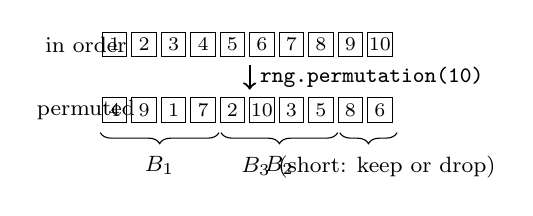
\begin{tikzpicture}[scale=0.52]
  % shuffle + batch diagram
  \foreach \i/\v in {0/1,1/2,2/3,3/4,4/5,5/6,6/7,7/8,8/9,9/10}{
    \draw (\i*0.72,2.4) rectangle (\i*0.72+0.6,3.0);
    \node[font=\scriptsize] at (\i*0.72+0.3,2.7) {\v};}
  \node[font=\footnotesize] at (-0.4,2.7) {in order};
  \foreach \i/\v in {0/4,1/9,2/1,3/7,4/2,5/10,6/3,7/5,8/8,9/6}{
    \draw (\i*0.72,0.8) rectangle (\i*0.72+0.6,1.4);
    \node[font=\scriptsize] at (\i*0.72+0.3,1.1) {\v};}
  \node[font=\footnotesize] at (-0.4,1.1) {permuted};
  \draw[->,thick] (3.6,2.2) -- (3.6,1.6) node[midway,right,font=\footnotesize]
    {\texttt{rng.permutation(10)}};
  % batches
  \draw[decorate,decoration={brace,amplitude=4pt,mirror}] (-0.05,0.55) -- (2.85,0.55)
    node[midway,below=5pt,font=\footnotesize] {$B_1$};
  \draw[decorate,decoration={brace,amplitude=4pt,mirror}] (2.9,0.55) -- (5.75,0.55)
    node[midway,below=5pt,font=\footnotesize] {$B_2$};
  \draw[decorate,decoration={brace,amplitude=4pt,mirror}] (5.8,0.55) -- (7.2,0.55)
    node[midway,below=5pt,font=\footnotesize] {$B_3$ (short: keep or drop)};
\end{tikzpicture}
\caption{The whole minibatch machinery of this book: permute the row indices
once, then hand out contiguous slices. The last batch is smaller than the rest
--- a decision, not an accident.}\label{fig:shuffle-batch}
\end{figure}

How much does vectorising actually buy? Enough to measure.

\lstinputlisting[language=Python,caption={\texttt{code/ch01/broadcast\_benchmark.py}: three workloads, three implementations each, median of warm runs.},label={lst:benchmark}]{code/ch01/broadcast_benchmark.py}

\lstinputlisting[numbers=none]{code/ch01/broadcast_benchmark.out.txt}

\begin{example}[Loop vs vectorised, priced]\label{ex:timing}
Strategy: time the same arithmetic three ways --- a Python loop over lists, a
NumPy call per row, and one vectorised expression.\par
\begin{solution}
On this machine the vectorised row-score (\texttt{X @ w}) runs $165\times$
faster than the per-row NumPy loop and $128\times$ faster than the Python
loop; the full table is in the output above and Figure~\ref{fig:timing}. Two
lessons, both worth internalising: the per-row \texttt{np.linalg.norm} loop is
the \emph{worst} of both worlds (Python-loop overhead \emph{plus} a fresh
array each iteration), and the gap only grows with $n$ --- your numbers will
differ from these, the ordering will not~\cite{harris2020}.
\end{solution}
\end{example}

\begin{figure}[ht]\centering
\begin{tikzpicture}
\begin{axis}[ybar,width=0.85\linewidth,height=5.2cm,bar width=15pt,
  symbolic x coords={scores-loop,scores-nprow,dist-loop,pairwise-loop},
  xtick=data,x tick label style={rotate=18,anchor=east,font=\scriptsize},
  ylabel={slowdown vs.\ vectorised ($\times$)},ymin=0,
  nodes near coords,nodes near coords style={font=\scriptsize},
  grid=major,grid style={gray!25}]
\addplot[fill=accentsoft,draw=accent] table[x=op,y=speedup] {figures/ch01/timing.dat};
\end{axis}
\end{tikzpicture}
\caption{Measured slowdowns from \texttt{broadcast\_benchmark.py} on a
$10^4\times4$ float64 matrix. The pairwise row compares a pure-Python double
loop against broadcasting on the first $2{,}000$ rows --- even at a size the
loop can finish, it is over $30\times$ slower.}\label{fig:timing}
\end{figure}

\begin{rulebox}[When not to vectorise]
Broadcasting builds the $(n,m,d)$ intermediate it needs. For pairwise
distances that is $8nmd$ bytes --- $10^4\times10^4\times4$ is already
$\sim$3~GB. When the intermediate stops fitting in memory, \emph{block} it:
vectorise inside a Python loop over row-chunks of a few thousand. The loop
runs a handful of times; the inner op stays in C.
\end{rulebox}

\begin{checkpoint}[Memory arithmetic]
How many bytes does the intermediate \texttt{(X[:, None, :] - X[None, :,
:])**2} need for $n=10^5$, $d=64$ float64? Is broadcasting the right tool
there? What is the fix?
\end{checkpoint}

\section{Data hygiene: duplicates, impossible values, units}\label{sec:hygiene}

Before any model touches a new file, three checks cost almost nothing and
catch most real-world dirt:

\begin{checklist}
\item \textbf{Duplicates}: \texttt{np.unique(X, axis=0)} --- exact twins are
  rare in honest measurement and common in scraped or merged data.
\item \textbf{Impossible values}: range-check each column against reality ---
  a bill length of $-2$~mm or $97.5$~mm, a mass of 0, an age of 212.
\item \textbf{Units}: read the schema \emph{and} the magnitudes. A height
  column mixing cm and m looks plausible row-by-row and is quietly nonsense.
  The column's summary statistics usually give the game away.
\end{checklist}

Why it matters beyond tidiness: duplicated rows break the assumption behind
every random split. If a row and its twin land on opposite sides of the
split, a memorising model has effectively seen some test answers during
training.

\lstinputlisting[language=Python,caption={\texttt{code/ch01/duplicates\_leak.py}: the duplicate-row leak, planted and measured.},label={lst:leak}]{code/ch01/duplicates_leak.py}

\lstinputlisting[numbers=none]{code/ch01/duplicates_leak.out.txt}

\begin{example}[The fake win]\label{ex:leak}
Strategy: plant duplicates, split randomly, and watch a 1-nearest-neighbour
classifier (ch.~3 formalises it) cash in free answers.\par
\begin{solution}
On \texttt{iris} the phantom gain is small ($+1.2$~pp) only because iris is
nearly separable --- there is little room left to inflate. On a harder
two-blob dataset the same bug buys $+11.5$~pp (Figure~\ref{fig:leak-bars}).
The fix costs one line \emph{before} the split: deduplicate
(\texttt{np.unique(X, axis=0)}) first, then split. This is the chapter's
failure-analysis item: \textbf{an accuracy is only as honest as the split
that produced it.}
\end{solution}
\end{example}

\begin{figure}[ht]\centering
\begin{tikzpicture}
\begin{axis}[ybar,width=0.6\linewidth,height=5.2cm,bar width=24pt,
  symbolic x coords={iris,blobs},xtick=data,
  ylabel={phantom gain (percentage points)},ymin=0,
  nodes near coords,nodes near coords style={font=\scriptsize},
  grid=major,grid style={gray!25}]
\addplot[fill=amberbg,draw=amber] table[x=scenario,y=gain] {figures/ch01/leak.dat};
\end{axis}
\end{tikzpicture}
\caption{What a duplicated row buys you: mean accuracy gained by splitting
\emph{before} deduplicating, over ten seeds each. The harder the task, the
bigger the fake win.}\label{fig:leak-bars}
\end{figure}

\begin{tripwire}[A clean number can be a leaked number]
\index{leakage}
Any step that looks at more rows than the training set --- deduplication,
imputation, scaling, vocabulary building --- must run \emph{before} the split
(if it is data-level, like dedup) or be fitted on training rows only (if it is
statistical, like a median). When in doubt, ask: \emph{would this information
exist at prediction time?}
\end{tripwire}

\section{Common mistakes}\label{sec:mistakes}

Every entry below has cost a real project real time.

\begin{description}
\item[Reading the shape backwards.] \texttt{(d, n)} instead of $(n, d)$:
  treating each feature as a sample. \emph{Fix:} say the shape aloud; row 0 is
  a sample.
\item[The silent $(n,n)$ broadcast.] Adding a $(n,1)$ column and a $(n,)$ row
  produces an $n\times n$ table instead of an element-wise op. \emph{Fix:}
  \texttt{b[:, None]}, or keep \texttt{keepdims=True} on the reduction that
  produced the vector.
\item[dtype truncation.] Assigning floats into an \texttt{int} array floors
  them silently; assigning \texttt{nan} into one raises \emph{or} wraps to a
  large integer depending on the path. \emph{Fix:} allocate
  \texttt{dtype=float} when the data is continuous; check
  \texttt{X.dtype} after any assembly.
\item[Shuffling $X$ and $\mathbf y$ differently.] Two permutations means every
  label is wrong and the model still trains happily. \emph{Fix:} permute
  \emph{indices} once; index everything with the same \texttt{perm}.
\item[Trusting \texttt{np.loadtxt} on dirty files.] It chokes on empty
  fields and mixed columns --- or worse, \texttt{genfromtxt} silently yields
  \texttt{nan} that then poisons means. \emph{Fix:} count \texttt{np.isnan}
  per column immediately after loading.
\item[Fitting statistics on all data.] A mean or median computed on
  train$+$test before splitting is a leak (small but real). \emph{Fix:}
  statistics on training rows only --- the pipeline order \emph{is} the bug
  fix.
\item[Losing the last batch.] \texttt{for k in range(n // B)} drops the
  remainder. \emph{Fix:} \texttt{range(0, n, B)} and accept a short final
  batch, or drop it deliberately and say so.
\item[Mutating a view.] \texttt{b = X[:, 0]; b /= b.max()} writes through into
  $X$ --- slices are views, not copies. \emph{Fix:} \texttt{.copy()} when you
  intend to modify.
\item[Treating ``missing'' as zero.] Filling a categorical hole with the
  all-zeros pattern makes missing indistinguishable from a real category.
  \emph{Fix:} missing gets its own column (or its own category), so the model
  can learn what absence means.
\end{description}

\section{Summary table}\label{sec:summary}

\begin{table}[ht]\centering\small
\begin{tabularx}{\linewidth}{@{}lYY@{}}
\toprule
\tablehead\thead{Object / step} & \thead{Meaning} & \thead{Idiom}\\
\midrule
$X\in\mathbb R^{n\times d}$ & design matrix, one row per sample &
\texttt{X.shape == (n, d)}\\
$\mathbf y$ & targets aligned to rows & \texttt{y.shape == (n,)}\\
broadcasting & size-1 axes stretch right-aligned &
\texttt{X - mu}, \texttt{A[:,None,:] - B[None,:,:]}\\
CSV load & strings first, convert per column &
\texttt{csv.reader} $\to$ \texttt{np.array(..., dtype=float)}\\
missing cells & count before repairing &
\texttt{np.isnan(X).sum(axis=0)}\\
categorical & nominal $\to$ one-hot, missing is a level &
\texttt{<missing>} column\\
shuffle & permute indices once, seed it &
\texttt{rng.permutation(n)}\\
batch & contiguous slices of the permuted order &
\texttt{X[perm[k:k+B]]}\\
vectorise & ops in C, not Python loops & \texttt{X @ w},
\texttt{np.linalg.norm(X, axis=1)}\\
dedup & before the split, always &
\texttt{np.unique(X, axis=0)}\\
leak check & statistics learned on train rows only &
\S\ref{sec:hygiene} tripwire\\
\bottomrule
\end{tabularx}
\caption{Chapter 1 cheat sheet: the shapes, the idioms, and the order of
operations that keeps the data honest.}\label{tab:cheat}
\end{table}

\section*{Exercises}
\addcontentsline{toc}{section}{Exercises}

\begin{exercise}[easy]
Predict, then verify: \texttt{np.array([1, 2, 3]) + 5},
\texttt{np.zeros((2, 3)) + np.ones(3)}, and the shapes of
\texttt{X[0]}, \texttt{X[:, 0]}, \texttt{X.T} for \texttt{X.shape == (150, 4)}.
\end{exercise}
\begin{exercise}[easy]
A $(5,1,4)$ array plus a $(3,4)$ array: write the output shape. Then a
$(2,3)$ plus a $(2,)$ --- does it broadcast? Give the result shape or the
error.
\end{exercise}
\begin{exercise}[easy]
What does \texttt{np.array([1.7, 2.3, 9.9], dtype=int)} produce, and why?
How would you make the rounding explicit instead?
\end{exercise}
\begin{exercise}[easy]
\texttt{np.loadtxt} meets the file \texttt{1.0,2.0\textbackslash n,3.0}:
what happens? And \texttt{np.genfromtxt}? Which behaviour is easier to live
with and why?
\end{exercise}
\begin{exercise}[easy]
In \texttt{onehot\_scratch.py}, a feature column with $k$ distinct levels and
no missing cells produces how many output columns? What if 5\% of its cells
are empty strings?
\end{exercise}
\begin{exercise}[medium]
Write \texttt{zscore(X)} in one line (column-wise standardisation), verify
\texttt{Z.mean(axis=0)} and \texttt{Z.std(axis=0)} on a random matrix, and
explain why \texttt{keepdims} is unnecessary here.
\end{exercise}
\begin{exercise}[medium]
Write \texttt{train\_val\_split(X, y, frac, seed)} returning
\texttt{(Xtr, ytr, Xval, yval)} using \texttt{default\_rng(seed)}. Why do we
pass \texttt{frac} rather than an absolute count? Give one call site where the
fraction matters.
\end{exercise}
\begin{exercise}[medium]
\texttt{genfromtxt} returned \texttt{nan} for the strings \texttt{""},
\texttt{"NA"}, and \texttt{"n/a"} but stored \texttt{-999} as a number.
Write the check that flags sentinel values like $-999$, and explain why
sentinels are more dangerous than NaNs.
\end{exercise}
\begin{exercise}[medium]
For $n=103$, $B=10$: how many batches does \texttt{range(0, n, B)} produce,
and of what sizes? Write \texttt{iter\_batches(perm, B)} yielding index
slices; should the generator shuffle, or take a permutation? Defend the
choice.
\end{exercise}
\begin{exercise}[medium]
A held-out penguin arrives with \texttt{island=Saunders}, a level your
codebook has never seen. What does your one-hot encoding from
\S\ref{sec:onehot} produce for it? Give two engineering answers (reject vs.\
all-zeros) and one situation each is right.
\end{exercise}
\begin{exercise}[medium]
Memory arithmetic: a $(10^6, 100)$ float64 matrix costs how much RAM? The
same data as float32? When is halving precision \emph{not} free?
\end{exercise}
\begin{exercise}[hard]
Implement \texttt{iter\_batches(X, y, B, seed)} as a generator that permutes
once per call and yields \texttt{(X\_b, y\_b)} including a possibly short
final batch. Prove: over $n$ samples, $\bigcup_k B_k$ is a partition of
$[n]$.
\end{exercise}
\begin{exercise}[hard]
Prove the broadcasting identity used in Listing~\ref{lst:load-iris}: for
$A\in\mathbb R^{n\times d}$ and centroids $C\in\mathbb R^{k\times d}$,
$\bigl(A[:,None,:]-C[None,:,:]\bigr)^2$ summed over the last axis equals the
$n\times k$ matrix of squared Euclidean distances
$\|\mathbf a_i-\mathbf c_j\|_2^2$. Where exactly does the stretch happen?
\end{exercise}
\begin{exercise}[hard]
Show that centring the columns of $X$ by \texttt{X - X.mean(axis=0)} is the
same as left-multiplying by the centring matrix $H=I_n-\frac1n\mathbf
1\mathbf 1^T$, i.e.\ $HX$. Conclude that centring twice is a no-op
($H^2=H$).
\end{exercise}
\begin{exercise}[hard]
A teammate's pipeline: load CSV $\to$ fill NaNs with the column median over
all rows $\to$ drop duplicate rows $\to$ shuffle $\to$ split $\to$ report
accuracy. Find the two leaks and reorder the pipeline to remove them. Which
leak did Listing~\ref{lst:leak} measure?
\end{exercise}
\begin{exercise}[hard]
Pairwise distances by blocking: write \texttt{pdist\_blocked(A, B, rows)}
that computes $\|a_i-b_j\|_2^2$ for all pairs using broadcasting inside a
loop over row-blocks of \texttt{A}. Show the memory bound it honours and
verify \texttt{allclose} against the single broadcast on small inputs.
\end{exercise}

\section*{Further reading}
\addcontentsline{toc}{section}{Further reading}

\begin{itemize}
\item NumPy documentation, \emph{NumPy: the absolute basics for beginners}
  (v2.5 manual), \url{https://numpy.org/doc/stable/user/absolute_beginners.html}.
  The official onboarding --- gentler than this chapter; read it alongside
  \S\ref{sec:numpy} if any idiom felt fast.
\item NumPy documentation, \emph{Broadcasting},
  \url{https://numpy.org/doc/stable/user/basics.broadcasting.html}. The three
  rules straight from the source, with the failing cases --- bookmark it, you
  will be back.
\item J.~VanderPlas, \emph{Python Data Science Handbook}, ch.~2, ``The Basics
  of NumPy Arrays'', \url{https://jakevdp.github.io/PythonDataScienceHandbook/02.02-the-basics-of-numpy-arrays.html}.
  Free online; intermediate. The vectorisation argument told properly, with
  ufuncs laid out one by one.
\item N.~P. Rougier, \emph{From Python to NumPy},
  \url{https://www.labri.fr/perso/nrougier/from-python-to-numpy/}. Free;
  intermediate-to-advanced. How a NumPy programmer thinks --- custom
  vectorisation as a design skill, not a trick.
\item Stanford CS231n, \emph{Python Numpy Tutorial},
  \url{https://cs231n.github.io/python-numpy-tutorial/}. A terse reference for
  the exact subset we use (arrays, broadcasting, indexing) --- keep it open in
  a tab for a week.
\item scikit-learn documentation, \emph{Common pitfalls}, esp.~§12.2 ``Data
  leakage'', \url{https://scikit-learn.org/stable/common_pitfalls.html}. The
  official checklist; our \S\ref{sec:loadleak} and \S\ref{sec:hygiene} are two
  items on it.
\item C.~R. Harris et al., ``Array programming with NumPy'', \emph{Nature}
  585 (2020), \url{https://www.nature.com/articles/s41586-020-2649-2}. Why the
  loop/vectorised gap is not an accident --- the architecture paper for the
  library you just used.
\item K.~B. Gorman, T.~D. Williams, W.~R. Fraser, ``Ecological sexual
  dimorphism and environmental variability within a community of Antarctic
  penguins'', \emph{PLOS ONE} 9(3) (2014),
  \url{https://journals.plos.org/plosone/article?id=10.1371/journal.pone.0090081}.
  Where the \texttt{penguins} data actually comes from --- worth it just for
  the field methods.
\item R.~A. Fisher, ``The use of multiple measurements in taxonomic
  problems'', \emph{Annals of Eugenics} 7(2) (1936),
  \url{https://doi.org/10.1111/j.1469-1809.1936.tb02137.x}. The iris paper.
  Historical interest: it is also the first linear discriminant analysis.
\end{itemize}

\begin{rulebox}[Watch instead]
If you would rather watch than read for a first pass (then come back and do
the exercises --- the exercises are where it becomes yours):
\begin{itemize}
\item \emph{Vectors | Chapter 1, Essence of linear algebra} ---
  \textbf{3Blue1Brown}, 9:51,
  \url{https://www.youtube.com/watch?v=fNk_zzaMoSs}. Matches \S\ref{sec:matrices}--\ref{sec:numpy}:
  the ``vector as an ordered list of numbers'' is exactly our $\mathbf x_i$.
  \textbf{Start here.}
\item \emph{Machine Learning Fundamentals: Cross Validation} ---
  \textbf{StatQuest with Josh Starmer}, 6:04,
  \url{https://www.youtube.com/watch?v=fSytzGwwBVw}. Matches
  \S\ref{sec:vectorise}--\ref{sec:hygiene}: why we split data at all; previews
  the evaluation protocol formalised in chapter~3.
\item \emph{Lecture 2 | Image Classification} ---
  \textbf{Stanford University School of Engineering} (CS231n), 59:31,
  \url{https://www.youtube.com/watch?v=OoUX-nOEjG0}. Matches \S\ref{sec:loading}--\ref{sec:hygiene}
  at course pace: the data-driven pipeline, a distance-based classifier like
  ours, and the train/val/test discipline. Long --- treat it as a week of
  commutes.
\end{itemize}
All three opened and verified 2026-10-11; none duplicates another.
\end{rulebox}

\section*{Notes}
\addcontentsline{toc}{section}{Notes}

\begin{enumerate}
\item Iris provenance: the 150-row iris set is Fisher's 1936
  measurements~\cite{fisher1936}; \texttt{penguins} is Gorman, Williams and
  Fraser's Palmer Station data~\cite{gorman2014}; we load both as CSVs from
  the seaborn-data collection~\cite{seaborn-data}.
\item The broadcasting rules and their failure modes are stated per the NumPy
  manual~\cite{npbroadcast}; the timing methodology (warm runs, medians)
  follows standard benchmarking practice --- rerun
  \texttt{broadcast\_benchmark.py} on your own machine before quoting numbers,
  as they are hardware-dependent.
\item The leakage taxonomy (normalise-then-split, fit-on-test) follows the
  scikit-learn pitfalls documentation~\cite{sklearnpitfalls}; this book
  returns to it formally in chapter~3.
\item A pedagogical note: applied courses such as fast.ai~\cite{fastai2022}
  put a working model before any mechanism. This book keeps the
  mechanism-first order --- Book 3 exists, so we can afford it --- but if you
  are impatient, the eight-line classifier in \S\ref{sec:loading} is the whole
  fast.ai lesson in miniature.
\item Version pins for this chapter's runs: Python~3.9, NumPy~2.0.2 ---
  recorded in \path{code/README.md}; dataset files live in \path{data/}.
\end{enumerate}

\section*{Hints and answers}
\addcontentsline{toc}{section}{Hints and answers}

\begin{description}
\item[1.1--1.5 (easy)] Work them in a Python prompt, not on paper --- the
  answer is the point of the exercise, the prompt is the point of the habit.
\item[1.6] \texttt{Z = (X - X.mean(0)) / X.std(0)}; means are $\approx0$,
  stds are $1$ up to float error.
\item[1.7] \texttt{k = int(frac * n)}; \texttt{perm = rng.permutation(n)};
  return slices. A fraction survives a dataset swap; a hardcoded count does
  not.
\item[1.8] Range-check per column (\texttt{(x < lo) | (x > hi)}), or treat the
  sentinel as missing before parsing. Sentinels are worse: \texttt{nan}
  trips \texttt{isnan}; $-999$ averages quietly into means.
\item[1.9] 11 batches: ten of 10, one of 3. Take \texttt{perm} in --- the
  caller owns the shuffle so $X$ and $\mathbf y$ stay aligned and
  reproducible.
\item[1.10] All-zeros in this design (Saunders matches no level column).
  Rejecting is right when the new level should change the model; all-zeros is
  right when ``unknown island'' is itself the signal.
\item[1.11] $10^6\times100\times8 \approx 800$~MB (float64), $\approx 400$~MB
  (float32). Halving precision is not free when small additive terms matter
  (e.g.\ accumulating $10^6$ squared errors) --- check dtype before blaming
  the model.
\item[1.12] Loop over \texttt{range(0, n, B)}; inside, slice both arrays with
  \texttt{perm[k:k+B]} and yield the pair. Disjoint contiguous slices of a
  permutation partition $[n]$.
\item[1.13] Expand the distance as a sum over coordinates: $\|\mathbf
  a_i-\mathbf c_j\|_2^2 = \sum_{t=1}^{d}(a_{it}-c_{jt})^2$ --- the last-axis
  sum \emph{is} that inner sum; the two \texttt{None} axes stretch $A$ over
  $j$ and $C$ over $i$.
\item[1.14] $H$ is symmetric idempotent: $H^2 = I - \frac2n\mathbf 1\mathbf
  1^T + \frac{n}{n^2}\mathbf 1\mathbf 1^T = H$. Centring is a projection ---
  Book 3's language.
\item[1.15] Median-fill on all rows leaks test statistics into training;
  dedup after split lets twins straddle the split --- the leak
  Listing~\ref{lst:leak} measured. Honest order: load $\to$ dedup $\to$ split
  $\to$ fit the median on \emph{train} $\to$ apply to both $\to$ evaluate.
\item[1.16] Loop over row-blocks of $A$ with broadcasting inside; the
  intermediate is at most $\texttt{rows}\times m\times d$ floats. It is the
  rulebox from \S\ref{sec:vectorise} made concrete.
\end{description}
